\section{Linear Transformations in $\mathbb{R}^n$}
\subsection{Definition}

\begin{definition}[Function]
A function $f:A \to B$ is a map the associates each value $a$ in the  
\emph{domain} $A$ with exactly one value $b$ in the \emph{codomain} $B$. 
We would write $f(a)=b$. We will call all the elements in $B$ actually mapped 
to by $f$ the \emph{image} of $A$ under $f$ and denote it 
$f(A)=\{ f(a):\text{ for } a \in A  \}$.
\end{definition}
\begin{example}$f:\mathbb{R} \to \mathbb{R}$ defined by $f(x)=x^2$ is a 
function. The domain  and the codomain are both $\mathbb{R}$ while the 
image is $f(\mathbb{R})=[0,\infty )$.
\end{example}
\begin{remark}
We are intentionally avoiding the term \emph{range} of a function because it is 
ambiguous. Some authors call the range the image and others call it the 
codomain.
\end{remark}
\begin{definition}[Linear Transformation]
\index{Linear Transformation!Definition}
A real \emph{linear transformation} is a function\\ 
$T: \mathbb{R}^n \to \mathbb{R}^m$ such that vector addition and scalar 
multiplication are preserved. That is, 
\begin{enumerate}
\item $T(\vec{v}+\vec{w})=T(\vec{v})+T(\vec{w})$ for all 
$\vec{v},\vec{w} \in \mathbb{R}^n$.\hfill \emph{(preserves vector addition)}
\item $T(r\vec{v})=r T(\vec{v})$ for all $\vec{v}\in \mathbb{R}^n$ 
and for $r \in \mathbb{R}$.\hfill \emph{(preserves scalar multiplication)}
\end{enumerate}
\end{definition}

\begin{proposition} If $A \in M_{m \times n}(\mathbb{R})$ then the function 
$T:\mathbb{R}^n \to \mathbb{R}^m$ defined by $T(\vec{v})=A\vec{v}$ is a linear 
transformation. This map is commonly referred to as $\vec{v} \to A\vec{v}$.
\label{prop:Av_is_linear}
\end{proposition}
\begin{proof}
Let $\vec{v},\vec{w} \in \mathbb{R}^n$ and $r \in \mathbb{R}$. 
We will start with scalar multiplication 
\begin{align*}
T(r\vec{v})
%=A\begin{bmatrix}av_1\\ \vdots \\ av_n\end{bmatrix}
&=[\vec{a}_1, \ldots, \vec{a}_n]
\begin{bmatrix}rv_1\\ \vdots \\  rv_n\end{bmatrix}\\
&=(r v_1)\vec{a}_1+\cdots+(r v_n)\vec{a}_n\\
&=r (v_1\vec{a}_1+\cdots+v_n\vec{a}_n)\\
&=r (A\vec{v})\\
&=r T(\vec{v}).
\end{align*}
Now we show vector addition is preserved:
\begin{align*}
T(\vec{v}+\vec{w})
%&=A\begin{bmatrix}v_1+w_1\\ \vdots \\ v_n+w_n\end{bmatrix}\\
&=[\vec{a}_1, \ldots, \vec{a}_n]\begin{bmatrix}v_1+w_1\\ \vdots \\ v_n+w_n\end{bmatrix}\\
&=(v_1+w_1)\vec{a}_1+\cdots+(v_n+w_n)\vec{a}_n\\
&=(v_1\vec{a}_1+\cdots+v_n\vec{a}_n)+(w_1\vec{a}_1+\cdots+w_n\vec{a}_n)\\
&=A\vec{v}+A\vec{w}\\
&=T(\vec{v})+T(\vec{w}).
\end{align*}
Note that the vector associative and distributive properties used above 
follow from the associative and distributive properties in $\mathbb{R}$ 
by applying them on each coordinate.

Since the choices of $\vec{v},\vec{w}$ and $r$ were arbitrary the proof 
works for all $\vec{v},\vec{w} \in \mathbb{R}^n$ and $r \in \mathbb{R}$.
\end{proof}

\begin{example} We will show that  map $T:\mathbb{R}^2 \to \mathbb{R}^3$ 
defined by 
$T\begin{bmatrix}v_1 \\ v_2 \end{bmatrix}=
\begin{bmatrix}v_1-3v_2\\v_2\\5v_1-3v_2\end{bmatrix}$
is a linear transformation.

Let $\vec{v},\vec{w} \in \mathbb{R}^n$. Then 
\begin{align*}
T(\vec{v}+\vec{w}) 
&= T\begin{bmatrix}v_1+w_1\\v_2+w_2\\v_3+w_3\end{bmatrix}\\
&= \begin{bmatrix}(v_1+w_1)-3(v_2+w_2)\\v_2+w_2\\5(v_1+w_1)-3(v_2+w_2)\end{bmatrix}\\
&= \begin{bmatrix}v_1-3v_2+w_1-3w_2\\v_2+w_2\\5v_1-3v_2+5w_1-3w_2\end{bmatrix}\\
&= \begin{bmatrix}v_1-3v_2\\v_2\\5v_1-3v_2\end{bmatrix}
+\begin{bmatrix}w_1-3w_2\\w_2\\5w_1-3w_2\end{bmatrix}\\
&= T(\vec{v})+T(\vec{w}).
\end{align*}
Thus $T$ preserves addition. Let $r\in \mathbb{R}$ then 
\begin{align*}
T(r\vec{v}) 
&= T\begin{bmatrix}rv_1\\rv_2\\rv_3\end{bmatrix}\\
&= \begin{bmatrix}rv_1-3rv_2\\rv_2\\5rv_1-3rv_2\end{bmatrix}\\
&= \begin{bmatrix}r(v_1-3v_2)\\r(v_2)\\r(5v_1-3v_2)\end{bmatrix}\\
&= r\begin{bmatrix}v_1-3v_2\\v_2\\5v_1-3v_2\end{bmatrix}\\
&= rT(\vec{v}).
\end{align*}
Thus $T$ is preserves scalar multiplication and is therefore a linear
transformation.
\end{example}

\begin{remark}
Notice that we write $T\begin{bmatrix}v_1\\v_2\\v_3\end{bmatrix}$ instead 
of  $T\left(\begin{bmatrix}v_1\\v_2\\v_3\end{bmatrix}\right)$ as a simple 
mater of convenience.
\end{remark}
\begin{proposition}
A linear transformation $T:\mathbb{R}^n \to \mathbb{R}^m$ has the property 
that $T(\vec{0}_n)=\vec{0}_m$ where $\vec{0}_n \in \mathbb{R}^n$ and 
$\vec{0}_m \in \mathbb{R}$ are the zero vectors.
\end{proposition}

Proof of the above proposition is an exercise.

\begin{example}The map $T:\mathbb{R}^3 \to \mathbb{R}^2$ defined by 
$T\begin{bmatrix}v_1 \\ v_2 \\ v_3\end{bmatrix}
=\begin{bmatrix*}[C]-7v_1+v_2 \\ v_1+v_2+3\end{bmatrix*}$ 
is not a linear transformation because $T(\vec{0})=\begin{bmatrix}0\\3\end{bmatrix}$.
\end{example}

\begin{restatable}{theorem}{lineartransformationequivalences}\label{thm:linear_transformation_equivalences}
Let $T:\mathbb{R}^n\to\mathbb{R}^m$ be a function. The following are equivalent:
\begin{enumerate}
\item $T$ is a linear transformation.
\item $T(a\vec{v}+b\vec{w})=aT(\vec{v})+bT(\vec{w})$ for all $a,b \in \mathbb{R}$ 
and $\vec{v},\vec{w} \in \mathbb{R}^n$.
\item $T(a_1\vec{v}_1+a_2\vec{v}_2+\cdots+a_k\vec{v}_k)=
a_1T(\vec{v}_1)+a_2T(\vec{v}_2)+\cdots+a_kT(\vec{v}_k)$ 
for all $a_i \in \mathbb{R}$ and $\vec{v}_i \in \mathbb{R}^n$ and $k$ a positive integer.
\end{enumerate}
\end{restatable}

\begin{proof}
We will show the equivalence of all three by showing $1 \implies 2$ and 
$2 \implies 3$ and $3 \implies 1$. 
Then the rest of the implications can be deduced working around the circle:\\
\begin{center}
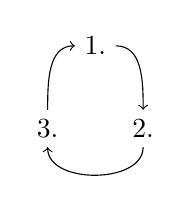
\begin{tikzpicture}[scale=.7]
\node[draw=none] (x) at (0,1) {1.};
\node[draw=none] (y) at (0.866025,-0.5) {2.};
\node[draw=none] (z) at (-0.866025,-0.5) {3.}; 
\draw[->] (x) to[in=90,out=0] (y);
\draw[->] (y) to[in=-90,out=-90] (z);
\draw[->] (z) to[in=180,out=90] (x);
\end{tikzpicture}
\end{center}
\begin{enumerate}
\item[$(1 \implies 2)$] Let $T$ be a linear transformation, 
$a,b \in \mathbb{R}$ and $\vec{v},\vec{w} \in \mathbb{R}^n$. Then
\begin{align*}
T(a\vec{v}+b\vec{w}) &= T(a\vec{v})+T(b\vec{w})\\
&= aT(\vec{v})+bT(\vec{w}).
\end{align*}
Since the choice of $a,b \in \mathbb{R}$ and $\vec{v},\vec{w} \in \mathbb{R}^n$
was arbitrary this equality holds for all choices of these values.

\item[$(2 \implies 3)$] We will use 2 multiple times to prove 3. 
To prove this part rigorously we need a technique 
called \textit{mathematical induction}. We present an informal proof here. \\

Let $a_1, \ldots, a_k \in \mathbb{R}$ and 
$\vec{v}_1,\ldots,\vec{v}_k \in \mathbb{R}^n$. We define 
$\vec{w}_1= a_1\vec{v}_1+a_2\vec{v}_2+\cdots+a_{k-1}\vec{v}_{k-1}$. Then we 
have 
\begin{align*}
T(a_1\vec{v}_1+\cdots+a_k\vec{v}_k)
&=T(\vec{w}_1+a_k\vec{v}_k)\\
&=T(\vec{w}_1)+a_{k}T(\vec{v}_k)\\
(\text{take }\vec{w}_2=a_1\vec{v}_1+a_2\vec{v}_2+\cdots+a_{k-2}\vec{v}_{k-2}, 
)&= T(\vec{w}_2+a_{k-1}\vec{v}_{k-1})+a_{k}T(\vec{v}_k)\\
&=T(\vec{w}_2)+a_{k-1}T(\vec{v}_{k-1})+a_{k}T(\vec{v}_k)\\
\text{ do this } k-3 \text{ times more } & \phantom{xx} \vdots \\
&=a_1T(\vec{v} _1)+\cdots+a_{k-1}T(\vec{v}_{k-1})+a_kT(\vec{v}_k).
\end{align*}

\item[$(3 \implies 1)$] Suppose 
$T(a_1\vec{v}_1+a_2\vec{v}_2+\cdots+a_k\vec{v}_k)=
a_1T(\vec{v}_1)+a_2T(\vec{v}_2)+\cdots+a_kT(\vec{v}_k)$ for all integers $k$ with $k \ge 1$.

Let $r\in \mathbb{R}$ and $\vec{v} \in \mathbb{R}^n$.
Then consider the $k=1$ case $a_1=r$ $\vec{v}_1=\vec{v}$. Then 
\begin{align*}
T(r\vec{v})&=T(a_1\vec{v}_1)\\
&=a_1T(\vec{v}_1)\\
&=rT(\vec{v}).
\end{align*}
Therefore $T$ preserves scalar multiplication.

Let $\vec{v},\vec{w} \in \mathbb{R}^2$. Consider the $k=2$ case where we let 
$a_1=a_2=1$, $\vec{v}_1=\vec{v}$ and $\vec{v}_2=\vec{w}$. Then
\begin{align*}
T(\vec{v}+\vec{w})&=T(a_1\vec{v}_1+a_2\vec{v}_2)\\
&=a_1T(\vec{v}_1)+a_2T(\vec{v}_2)\\
&=1T(\vec{v})+1T(\vec{w})\\
&=T(\vec{v})+T(\vec{w}).
\end{align*}
Thus $T$ also preserves vector addition and is therefore a 
linear transformation.
\end{enumerate}
\end{proof}

\subsubsection{Exercises}
%\addcontentsline{toc}{subsubsection}{Exercises}


\subsection{The Standard Matrix of a Linear Transformation}


\begin{definition}
\index{Linear Transformation!The Standard Matrix}
Let  $T:\mathbb{R}^n \to \mathbb{R}^m$ be a linear transformation. If there 
exists $A \in M_{m\times n}(\mathbb{R})$ such that $T(\vec{v})=A\vec{v}$ then 
$A$ is called \emph{the standard matrix} of $T$.
\end{definition}

\begin{theorem} Every linear transformation $T:\mathbb{R}^n \to \mathbb{R}^m$ 
has a standard matrix $A=[\vec{a}_1,\vec{a}_2, \ldots, \vec{a}_n]$. In fact,
$\vec{a}_k=T(\vec{e}_k)$ for each integer $k$ with $1 \le k \le n$ 
where $\mathcal{E}=\{\vec{e}_1,\vec{e}_2,\ldots,\vec{e}_n\}$ are the 
standard basis for $\mathbb{R}^n$.\label{thm:standard_matrix}
\end{theorem}

\begin{proof}
It suffices to show that $T(\vec{v})=A\vec{v}$ for all 
$\vec{v} \in \mathbb{R}^n$.
Let $\vec{v} \in \mathbb{R}^n$ be an arbitrary, but fixed, vector. By 
Proposition~\ref{prop:e_k_spans_Rn} $\vec{v}$ is a linear combination of the 
standard basis. In fact, it can be written:
\[
\vec{v}=v_1\vec{e}_1+v_2\vec{e}_2+\cdots+v_n\vec{e}_n
\]
where the each $v_k$ is the $k^{\text{th}}$ coordinate of $\vec{v}$. Thus
\begin{align*}
T(\vec{v}) 
&=T(v_1\vec{e}_1+v_2\vec{e}_2+\cdots+v_n\vec{e}_n)\\
&=v_1T(\vec{e}_1)+v_2T(\vec{e}_2)+\cdots+v_nT(\vec{e}_n)\\
&=v_1\vec{a}_1+v_2\vec{a}_2+\cdots+v_n\vec{a}_n\\
&=[\vec{a}_1,\vec{a}_2,\ldots,\vec{a}_n]
\begin{bmatrix}v_1\\v_2\\\vdots\\v_n\end{bmatrix}\\
&=A\vec{v}.
\end{align*}
\end{proof}

\begin{example} Let us find the standard matrix for the linear transformation
$T:\mathbb{R}^2 \to \mathbb{R}^3$ 
defined by 
$T\begin{bmatrix}v_1 \\ v_2 \end{bmatrix}=
\begin{bmatrix}v_1-3v_2\\v_2\\5v_1-3v_2\end{bmatrix}$.
Since the domain is $\mathbb{R}^2$ we use the standard basis 
$\mathcal{E}=\{\vec{e}_1,\vec{e}_2\}$ for $\mathbb{R}^2$. 
\begin{alignat*}{9}
\vec{a}_1
&=T(\vec{e}_1) 
&= T\begin{bmatrix}1 \\ 0\end{bmatrix} &=\begin{bmatrix}1\\0\\5\end{bmatrix}
&\hspace*{1.5cm} &\vec{a}_2
&=T(\vec{e}_2) 
&= T\begin{bmatrix}0 \\ 1\end{bmatrix} 
&=\begin{bmatrix*}[C]-3\\1\\-3\end{bmatrix*}.
\end{alignat*}
So $A=\begin{bmatrix*}[c]1 & -3 \\0 & 1 \\5 & -3\\\end{bmatrix*}$. 
We can test our work simply by multiplying:
\[
A\begin{bmatrix}v_1 \\ v_2 \end{bmatrix}
=\begin{bmatrix*}[c]1 & -3 \\0 & 1 \\5 & -3\\\end{bmatrix*}
\begin{bmatrix}v_1 \\ v_2 \end{bmatrix}
=\begin{bmatrix}
v_1-3v_2 \\ v_2 \\ 5v_1-3v_2
\end{bmatrix}.
\]
\end{example}
By combining Theorem \ref{thm:standard_matrix} and 
Proposition \ref{prop:Av_is_linear} we can use the existence of a standard 
matrix to prove or disprove a particular function is linear. 
\begin{example}
Consider $T:\mathbb{R}^4 \to \mathbb{R}$ defined by
\[
T\begin{bmatrix}v_1 \\ v_2 \\ v_3 \\ v_4 \end{bmatrix}=5v_1-3v_3+v_4.
\]
Then $T(\vec{e}_1)=5$, $T(\vec{e}_2)=0$, $T(\vec{e}_3)=-3$ and $T(\vec{e}_4)=1$ 
so $A=\begin{bmatrix}5 & 0 & -3 & 1\end{bmatrix}$.
By checking, 
\[
\begin{bmatrix}5 & 0 & -3 & 1\end{bmatrix}
\begin{bmatrix}v_1 \\ v_2 \\ v_3 \\ v_4 \end{bmatrix}
=5v_1+0v_2-3v_3+v_4=T(\vec{v})
\]
we prove that $T$ can be written as a matrix-vector product and therefore is 
a linear transformation.
\end{example}

\begin{example}
Consider the function $T:\mathbb{R}^3\to \mathbb{R}^2$ via
\[
T\begin{bmatrix}v_1 \\ v_2 \\ v_3 \end{bmatrix}
=\begin{bmatrix}3v_1-2v_2^2 \\ 3+v_2\end{bmatrix}.
\]
This function is not linear but we can still make what looks like a
matrix for it:
\[
T(\vec{e}_1)=\begin{bmatrix}3\\3\end{bmatrix},  
T(\vec{e}_2)=\begin{bmatrix*}[C]-2\\4\end{bmatrix*}, 
\text{ and }T(\vec{e}_3)=\begin{bmatrix}0\\3\end{bmatrix}.
\]
This might lead us to believe that $A=\begin{bmatrix*}[C] 3 & -2 & 
0 \\ 3 & 4 & 3 \end{bmatrix*}$. However, checking the multiplication reveals 
the problem,
\[A\vec{v}=\begin{bmatrix}3v_1-2v_2\\3v_1+4v_2+3v_3\end{bmatrix}
\neq \begin{bmatrix}3v_1-2v_2^2 \\ 3+v_2\end{bmatrix}.\]
Therefore $T$ does not have a standard matrix so is not a linear 
transformation.
\end{example}
\subsubsection{Exercises}
%\addcontentsline{toc}{subsubsection}{Exercises}

\begin{exercise} If the following function is linear transformation find its standard matrix. Use this matrix to determine if the function is a linear transformation.
\begin{inparaenum}[a)]
\item $S\begin{bmatrix}a\\b\\c\end{bmatrix}=\begin{bmatrix}3a-2b \\ 2a-c \\ a \\ b-c \\ c \end{bmatrix}$ \hfill
\item $T\begin{bmatrix} y_1 \\ y_2 \end{bmatrix} = \begin{bmatrix} y_1 \\ 3 y_1 \end{bmatrix}$ \hfill {} \\
\item $R\begin{bmatrix}x \\ y \\ z \end{bmatrix} = 3x+2y-z$ \hfill 
\item $M\begin{bmatrix}x \\ y \\ z \end{bmatrix} = 3x+7$ \hfill {} \\
\item $T\begin{bmatrix}x \\ y \\ z \end{bmatrix} = \begin{bmatrix} x+y+z \\ y+z \\ 3z^2 \end{bmatrix}$ \hfill 
\item $S(a)=\begin{bmatrix*}[C] 7a \\ 0 \\ -a \end{bmatrix*}$ \hfill {} \\
\item $R\begin{bmatrix}a \\ b \\ c \end{bmatrix} =\begin{bmatrix*}[C] 2a \\ 3b \\ 0 \\ -c \end{bmatrix*}$ \hfill
\item $M \begin{bmatrix}x_1\\ x_2 \\ x_3\end{bmatrix}=\begin{bmatrix}x_2\\ x_1 \\ x_3\end{bmatrix}$ \hfill {} \\
\end{inparaenum}
\end{exercise}

\subsection{Compositions of Linear Transformations}
\index{Linear Transformation!Compositions}
Consider two linear transformations 
$T:\mathbb{R}^n\ \to \mathbb{R}^m$ and $S:\mathbb{R}^p \to \mathbb{R}^n$. 
Since the domain of $T$ is equal to the codomain of $S$ we define the 
composition of function $T \circ S: \mathbb{R}^p \to \mathbb{R}^m$ by 
$T \circ S(\vec{v})=T(S(\vec{v}))$ for all $v \in \mathbb{R}^p$. 
the following theorem shows that the composition is linear.

\begin{theorem}
Let $T:\mathbb{R}^n\ \to \mathbb{R}^m$ and $S:\mathbb{R}^p \to \mathbb{R}^n$ 
be linear transformations. Then the composition 
$T\circ S:\mathbb{R}^p \to \mathbb{R}^m$ is also a linear transformation.
\end{theorem}

\begin{proof}
Let $\vec{v},\vec{w} \in \mathbb{R}^p$ and $a,b \in \mathbb{R}$. 
We then apply the linearity properties of $S$ then $T$ in turn.
\begin{align*}
T\circ S(a\vec{v}+b\vec{w})&=T(S(a\vec{v}+b\vec{w}))\\
&=T(aS(\vec{v})+bS(\vec{w}))\\
&=aT(S(\vec{v}))+bT(S(\vec{w}))\\
&=aT\circ S(\vec{v})+bT\circ S(\vec{w}).
\end{align*}
Therefore $T\circ S$ is a linear transformation.
\end{proof}
Next we may ask, since composition of linear transformation is linear, what
can we say about the standard matrix of a composition?
\begin{example}
Let $T:\mathbb{R}^2 \to \mathbb{R}^3$ and $S:\mathbb{R}^4 \to \mathbb{R}^2$
defined by $T(\vec{v})=A\vec{v}$ and $S(\vec{w})=B\vec{w}$ with
\begin{gather*}
A=\begin{bmatrix*}[C]
1 & 2 \\
-1 & 1 \\
3 & 2 
\end{bmatrix*}
B=\begin{bmatrix*}[C]
-3 & 0 & 2 & -7 \\
1 & 1 & -1 & 0 
\end{bmatrix*}
\end{gather*}
$T\circ S:\mathbb{R}^4 \to \mathbb{R}^3$ so we just need to consider it's 
action on the basis $\{\vec{e}_1,\vec{e}_2,\vec{e}_3,\vec{e}_4\}$.\\
%
$T\circ S(\vec{e}_1)=T(S(\vec{e}_1))=T(B\vec{e}_1)=A(B\vec{e}_1)
=A\begin{bmatrix*}[C]-3 \\ 1\end{bmatrix*}
=\begin{bmatrix*}[C] -1 \\ 4 \\ -7\end{bmatrix*}
$\\
$T\circ S(\vec{e}_2)=T(S(\vec{e}_2))=T(B\vec{e}_2)=A(B\vec{e}_2)
=A\begin{bmatrix}0 \\ 1\end{bmatrix}
=\begin{bmatrix} 2 \\ 1 \\ 2\end{bmatrix}
$\\
$T\circ S(\vec{e}_3)=T(S(\vec{e}_3))=T(B\vec{e}_3)=A(B\vec{e}_3)
=A\begin{bmatrix*}[C]2 \\ -1\end{bmatrix*}
=\begin{bmatrix*}[C] 0 \\ -3 \\ 4\end{bmatrix*}
$\\
$T\circ S(\vec{e}_4)=T(S(\vec{e}_4))=T(B\vec{e}_4)=A(B\vec{e}_4)
=A\begin{bmatrix*}[C]-7 \\ 0\end{bmatrix*}
=\begin{bmatrix*}[C] -7 \\ 7 \\ -21 \end{bmatrix*}
$. This gives a a standard matrix of 
\[\begin{bmatrix*}[C]
-1 & 2 &  0 & -7 \\
 4 & 1 & -3 &  7 \\
-7 & 2 &  4 & -21 
\end{bmatrix*}.
\]
But more importantly we notice that the standard matrix was made of 
$[A\vec{b}_1, A\vec{b}_2, A\vec{b}_3,A\vec{b}_4]$ where 
$B=[\vec{b}_1,\vec{b}_2, \vec{b}_3,\vec{b}_4]$. Also notice that we write 
$A(B\vec{v})$ quite a bit. In this spirit we have the following definition.
\end{example}


\begin{definition}[Matrix-Matrix Multiplication]
Let $A \in M_{m \times n}$ and $B \in M_{n \times p}$ we define the matrix 
product $AB=[A\vec{b}_1,A\vec{b}_2,\ldots,A\vec{b}_m]$.
\end{definition}

\begin{remark} We have two remarks about the definition above. 
\begin{enumerate}
\item The matrix product $AB$ only exists when the number of columns in $A$ is
equal to the number of rows in $B$. 
\item This definition is based on compositions of functions. Composite 
operations rarely commute (like putting on your socks and shoes). Thus in 
general $AB$ is not usually equal to $BA$. In fact only one may exist.
\end{enumerate}
\end{remark}

\begin{example}
Some examples here...
\end{example}

\begin{theorem} 
Let $T:\mathbb{R}^n \to \mathbb{R}^m$ and $S:\mathbb{R}^p \to \mathbb{R}^n$
defined by $T(\vec{v})=A\vec{v}$ and $S(\vec{w})=B\vec{w}$ for some
$A \in M_{m\times n}(\mathbb{R})$ and $B \in M_{n\times p}(\mathbb{R})$.
Then the standard matrix of $T \circ S$ is $AB$.
\end{theorem}
\begin{proof}
The composition $T \circ S$ is a linear transformation from $\mathbb{R}^p$ to 
$\mathbb{R}^m$. Let $B=[\vec{b}_1,\vec{b}_2,\ldots,\vec{b}_p]$  and 
$\mathcal{E}=\{\vec{e}_1,\vec{e}_2,\ldots,\vec{e}_p\}$ be the standard basis. 
Let  $k$ be an arbitrary integer with $1 \le k \le p$. Then 
\[
B\vec{e}_k
=0\vec{b}_1+\cdots+0\vec{b}_{k-1}+1\vec{b}_k+0\vec{b}_{k+1}+\cdots+0\vec{b}_p
=\vec{b}_k.
\]
Thus we can expand 
\[
T \circ S(\vec{e}_k) =T(S(\vec{e}_k))=T(B(\vec{e}_k))=T(\vec{b}_k)=A\vec{b}_k.
\]
Since $k$ was arbitrary this holds for all $k$ with $1 \le k \le p$. 
Therefore, the standard matrix for $T \circ S$ is 
$[A\vec{b}_1,\ldots, A\vec{b}_p]$ which is $AB$, by definition.
\end{proof}

\subsubsection{Exercises}
%\addcontentsline{toc}{subsubsection}{Exercises}
\begin{exercise}
Consider the linear transformations 
$T(\vec{v})=\begin{bmatrix*}[C]
1  & 3  & 5 \\
-1 & 0  & 10 \\
\end{bmatrix*}\vec{v}$

and $S(\vec{w})=\begin{bmatrix*}[C]
1 & 2 \\
-3 & 4 \\
-1 & -1
\end{bmatrix*}$.
\begin{enumerate}
\item Is it possible to compose the functions $T \circ S$? Why? If yes find the standard matrix of $T \circ S$
\item Is it possible to compose the functions $S \circ T$? Why? If yes find the standard matrix of $S \circ T$
\end{enumerate}
\end{exercise}





\clearpage

\subsection{Row Vectors, Transpose and Duality}

Sometimes it is useful for us to deal with row vectors:

$$
\mathbb{R}_\text{row}^n=\left\{ 
\begin{bmatrix}v_1 & v_2 & \cdots & v_n\end{bmatrix}
\mid v_i \in \mathbb{R} \text{ for all } i\ \right\}
$$

We can also think of row vectors as the set of $1 \times n $ matrices, that is $\mathbb{R}^n_\text{row} = M_{1 \times n}(\mathbb{R})$.

For $A \in  M_{n \times m}(\mathbb{R})$ we can write $A$ in terms of its row vectors $\vec{r}_1, \vec{r}_2, \ldots, \vec{r}_n \in \mathbb{R}^n_\text{row}$ in the 
following way

$$
A=\begin{bmatrix}\vec{r}_1 \\ \vec{r}_2 \\ \vdots \\ \vec{r}_n \end{bmatrix}=
\begin{bmatrix}
a_{11} & a_{12} & \cdots & a_{1m} \\
a_{21} & a_{22} & \cdots & a_{2m} \\
\vdots & \vdots & \ddots & \vdots \\
a_{n1} & a_{n2} & \cdots & a_{nm} \\
\end{bmatrix}
$$

Where for each $k$, the row vector $\vec{r}_k=\begin{bmatrix}a_{k1} & a_{k2} & \cdots & a_{km}\end{bmatrix}$

For a $v \in \mathbb{R}_\text{row}^n$ we define left vector-matrix multiplication by a matrix $A\in M_{n \times m}(\mathbb{R})$ with row vectors 
$\vec{r}_1, \ldots, \vec{r}_n \in \mathbb{R}^m_\text{row}$ to be:


$$
\begin{bmatrix}v_1 & v_2 & \cdots & v_n\end{bmatrix}\begin{bmatrix}\vec{r}_1 \\ \vec{r}_2 \\ \vdots \\ \vec{r}_n\end{bmatrix}
=v_1\vec{r}_1+v_2\vec{r}_2+ \cdots + v_n\vec{r}_n 
$$

\begin{example}
$$
\begin{bmatrix}1 & 2 & 3 \end{bmatrix} \begin{bmatrix*}[C] 1 & 1 & 1 & 1 \\ 0 & 1 & 0 & 1 \\ 0 & -1 & 0 & 1 \end{bmatrix*}
=1 \begin{bmatrix}1 & 1 & 1 & 1\end{bmatrix}+2\begin{bmatrix}0 & 1 & 0 & 1\end{bmatrix}+3\begin{bmatrix}0 & -1 & 0 & 1 \end{bmatrix}
=\begin{bmatrix} 1 & 0 & 1 & 6 \end{bmatrix}
$$
%
\end{example}

\begin{proposition}
For $\vec{v} \in \mathbb{R}^n_\text{row}$ and $A \in M_{n \times m}$ left vector-matrix multiplication $\vec{v}A$ is the same as the matrix-matrix multiplication 
acheiced by considering $\vec{v}$ as a $1 \times n$ matrix.
\end{proposition}
\begin{proof}
Let $A=[a_{ij}]=[\vec{a}_1, \vec{a}_2, \cdots, \vec{a}_m]=
\begin{bmatrix}
\vec{r}_1\\
\vec{r}_2\\
\vdots \\ 
\vec{r}_n
\end{bmatrix}=
\begin{bmatrix}
a_{11} & a_{12} & \cdots & a_{1m}\\
a_{21} & a_{22} & \cdots & a_{2m}\\
\vdots & \vdots & \ddots & \vdots\\
a_{n1} & a_{n2} & \cdots & a_{nm}\\
\end{bmatrix}
$.

As a matrix product:
\begin{align*}
\vec{v}A&=[\vec{v}\vec{a}_1, \vec{v}\vec{a}_2, \ldots, \vec{v}\vec{a}_m]\\
&=[v_1a_{11}+v_2a_{21}+\cdots+v_na_{n1}, v_1a_{12}+v_2a_{22}+\cdots+v_na_{n2}, \ldots, v_1a_{1m}+v_2a_{2m}+\cdots+v_na_{nm}]
\end{align*}

The left vector matrix product is:
\begin{align*}
\vec{v}A &=v_1\vec{r}_1+v_2\vec{r}_2+\cdots+v_n\vec{r}_n\\
&=[v_1a_{11}, v_1a_{12}, \ldots, v_1a_{1m}]+[v_2a_{21}, v_2a_{22}, \ldots, v_2a_{2m}]+\cdots+[v_na_{n1}, v_na_{n2}, \ldots, v_na_{nm}]\\
&=[v_1a_{11}+v_2a_{21}+\cdots+v_na_{n1}, v_1a_{12}+v_2a_{22}+\cdots+v_na_{n2}, \ldots, v_1a_{1m}+v_2a_{2m}+\cdots+v_na_{nm}]
\end{align*}
\end{proof}

We define linear transformations to be functions $T:\mathbb{R}^m_\text{row} \to \mathbb{R}^n_\text{row}$ that preserve vector addition and scalar multiplication. 

\begin{definition}[The Transpose]
For $m \times n$ matrix $$A=[a_{ij}]=
\begin{bmatrix}
a_{11} & a_{12} & \cdots & a_{1n} \\
a_{21} & a_{22} & \cdots & a_{2n} \\
\vdots & \vdots & \ddots & \vdots \\
a_{m1} & a_{m2} & \cdots & a_{mn} 
\end{bmatrix}
$$ 
we define \textbf{the transpose} to be an $n \times m$ matrix  
$$A^T=[a_{ji}]=
\begin{bmatrix}
a_{11} & a_{21} & \cdots & a_{m1} \\
a_{12} & a_{22} & \cdots & a_{m2} \\
\vdots & \vdots & \ddots & \vdots \\
a_{1n} & a_{2n} & \cdots & a_{nm} 
\end{bmatrix}$$ 
\end{definition}

\begin{remark}
The transpose works on vectors too since $\mathbb{R}^n=M_{1 \times n}(\mathbb{R})$ and $\mathbb{R}^n_\text{row}=M_{n \times 1}(\mathbb{R})$. 
\end{remark}

\begin{example}
\[
\begin{bmatrix}
1 \\
2 \\
3 \\
\end{bmatrix}^T
=\begin{bmatrix}
1 & 2 & 3
\end{bmatrix}
\]
\end{example}

\begin{example}
\[
\begin{bmatrix}
1 & 2 & 3 \\
4 & 5 & 6 
\end{bmatrix}^T
=\begin{bmatrix}
1 & 4 \\
2 & 5 \\
3 & 6 \\
\end{bmatrix}
\]
\end{example}

\begin{proposition}
Let $A$ and $B$ be matrices and $r$ a scalar. Then 
\begin{enumerate}
\item $(A^T)^T=A$
\item $(A+B)^T=A^T+B^T$ whenever $A$ and $B$ are both $m \times n$ matrices
\item $(rA)^T=r(A^T)$
\item $(AB)^T=B^TA^T$ whenever $A$ is an $m \times n$ and $B$ is an $n \times p$
\item If $\vec{r}_i$ is the $i$-th row of $A$ if and only if $\vec{r}_i^T$ is the $i$-th column of $A^T$ 
\item If $\vec{a}_i$ is the $i$-th column of $A$ if and only if $\vec{a}_i^T$ is the $i$-th row of $A^T$ 
\end{enumerate}
\end{proposition}
